\documentclass[12pt]{article}

% Preamble
\usepackage[utf8]{inputenc}
\usepackage{graphicx}
\usepackage{hyperref}
\usepackage{amsmath}
\usepackage{amsfonts}
\usepackage{amssymb}
\usepackage{xcolor}
\usepackage[left=3cm, right=3cm, top=2cm, bottom=2cm]{geometry}

\title{CA 2023 Lab2}
\author{Yu-Xiang Luo}
\date{\today}

% Document starts here
\begin{document}

\maketitle

\section*{\texttt{ALU.v}}
In \textbf{\texttt{ALU.v}}, we do the operation to data1 and data2, and the operation is based on \texttt{ALUCtrl\_i}, and we output back to the \textbf{\texttt{CPU.v}}.\\
\[
	\text{\small \textcolor{red}{\textbf{About the code:} define in ALU.v could be arbitary, just make sure it maps correctly to \texttt{ALU\_Ctrl.v}}}
\]

\section*{\texttt{ALU\_Control.v}}
In \textbf{\texttt{ALU\_Control.v}}, we decide the \textit{\texttt{ALUCtrl}} by \textit{\texttt{ALUop}} and \texttt{\textit{funct}}.

\section* {\texttt{Branch.v}}
In \texttt{\textbf{Branch.v}}, it outputs \textit{\texttt{Flush}}, which is the same as \textit{\texttt{ID\_FlushIF}}, so that \texttt{\textbf{ID\_IF.v}} knows when to flush, the same output is used to the \texttt{MUX\_PC} later to decide whether branch.

\newpage
\section* {\texttt{CPU.v}}
It connects all modules together, by the rule of the pipelined datapath figure in spec.\\ \\
\fbox{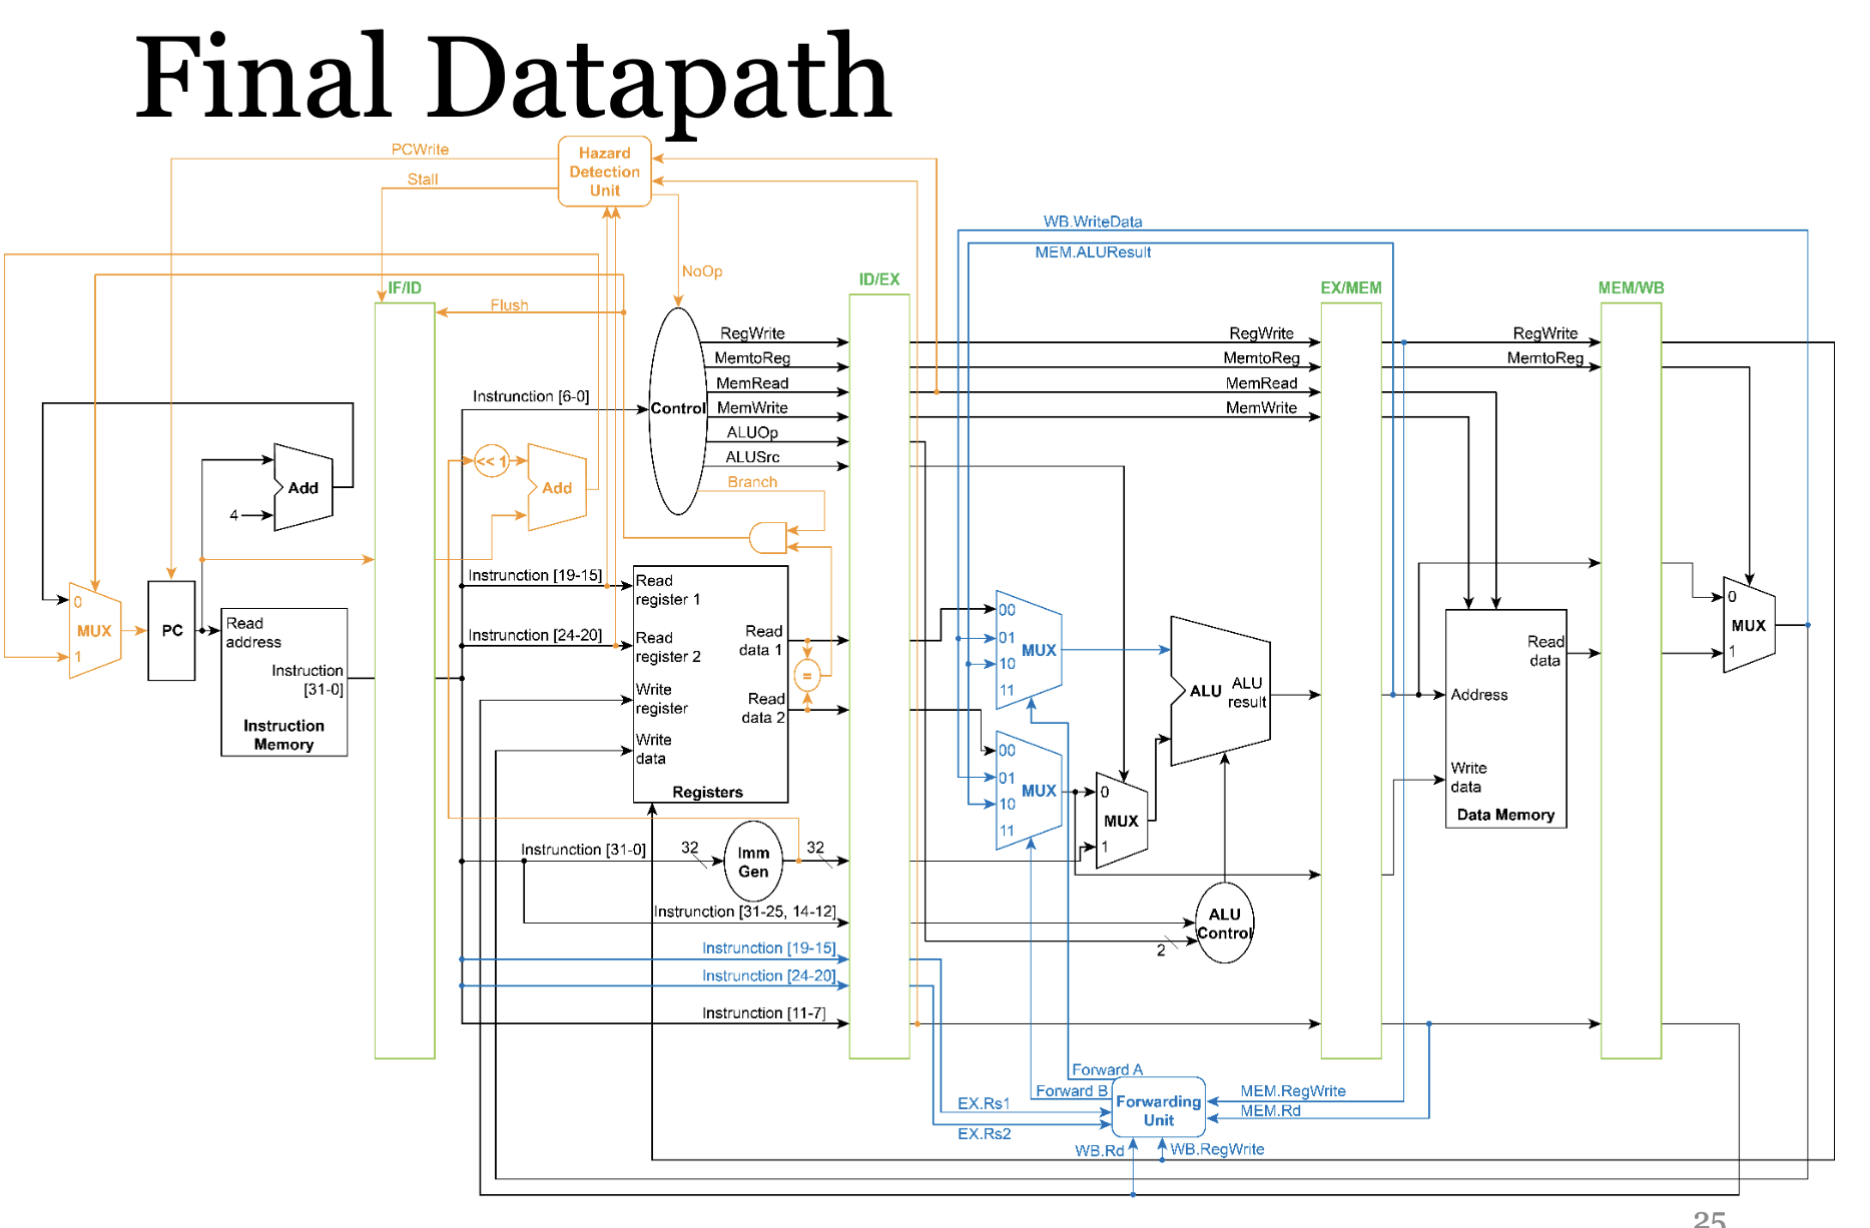
\includegraphics[width=\textwidth]{./datapath.png}}

\section* {\texttt{Control.v}}
Same as \textbf{\texttt{lab\_1}}, assign the control wire with the correct signal.

\section* {\texttt{ID\_EX.v, EX\_MEM.v, MEM\_WB.v}}
These module are stored to cut the datapath to multiple cycle, by updating the registers' value at the rising edge of clk.

\section* {\texttt{Forwarding.v}}
This module check two hazard, EX hazard is easy since we only have to check if \texttt{MEM\_RegWrite} and \texttt{MEM\_RDaddr} are both true, then recognize rs1 or rs2 hazard and store to ForwardA, ForwardB separately. The MEM hazard is alike, check \texttt{WB\_RegWrite} and \texttt{WB\_RDaddr} first, also, MEM hazard must check \texttt{MEM\_RegWrite} since EX hazard is already been handled.

\section* {\texttt{Hazard\_Detection.v}}
We all know load-use needs stall to prevent hazard, so this module checks if there's a load-use hazard by checking the control and the address of rs1 and rs2.

\section* {\texttt{Adder.v, MUX.v, Sign\_Extend.v}}
These are simple, no additional explanation.
\end{document}

